\documentclass{beamer}
\beamertemplatenavigationsymbolsempty
\usecolortheme{beaver}
\setbeamertemplate{blocks}[rounded=true, shadow=true]
\setbeamertemplate{footline}[page number]
%
% packages
\usepackage{amsmath,amssymb}
\usepackage{graphicx}
\usepackage{hyperref}

% directory of figures
%\graphicspath{ {figs} }

% latin bold lower
\newcommand{\ba}{\mathbf{a}}
\newcommand{\bc}{\mathbf{c}}
\newcommand{\be}{\mathbf{e}}
\newcommand{\bh}{\mathbf{h}}
\newcommand{\bp}{\mathbf{p}}
\newcommand{\bt}{\mathbf{t}}
\newcommand{\bs}{\mathbf{s}}
\newcommand{\bu}{\mathbf{u}}
\newcommand{\bv}{\mathbf{v}}
\newcommand{\bw}{\mathbf{w}}
\newcommand{\bx}{\mathbf{x}}
\newcommand{\by}{\mathbf{y}}
\newcommand{\bz}{\mathbf{z}}
\newcommand{\bm}{\mathbf{m}}

% latin bold upper
\newcommand{\bA}{\mathbf{A}}
\newcommand{\bB}{\mathbf{B}}
\newcommand{\bC}{\mathbf{C}}
\newcommand{\bI}{\mathbf{I}}
\newcommand{\bJ}{\mathbf{J}}
\newcommand{\bL}{\mathbf{L}}
\newcommand{\bM}{\mathbf{M}}
\newcommand{\bP}{\mathbf{P}}
\newcommand{\bQ}{\mathbf{Q}}
\newcommand{\bR}{\mathbf{R}}
\newcommand{\bT}{\mathbf{T}}
\newcommand{\bU}{\mathbf{U}}
\newcommand{\bV}{\mathbf{V}}
\newcommand{\bW}{\mathbf{W}}
\newcommand{\bX}{\mathbf{X}}
\newcommand{\bY}{\mathbf{Y}}
\newcommand{\bZ}{\mathbf{Z}}

% latin cal upper
\newcommand{\cF}{\mathcal{F}}
\newcommand{\cG}{\mathcal{G}}
\newcommand{\cI}{\mathcal{I}}
\newcommand{\cL}{\mathcal{L}}
\newcommand{\cM}{\mathcal{M}}
\newcommand{\cN}{\mathcal{N}}
\newcommand{\cS}{\mathcal{S}}
\newcommand{\cT}{\mathcal{T}}
\newcommand{\cW}{\mathcal{W}}
\newcommand{\cX}{\mathcal{X}}
\newcommand{\cZ}{\mathcal{Z}}

% latin bb upper
\newcommand{\bbE}{\mathbb{E}}
\newcommand{\bbI}{\mathbb{I}}
\newcommand{\bbP}{\mathbb{P}}
\newcommand{\bbR}{\mathbb{R}}
\newcommand{\bbX}{\mathbb{X}}
\newcommand{\bbY}{\mathbb{Y}}
\newcommand{\bbW}{\mathbb{W}}

% greek bold lower
\newcommand{\bepsilon}{\boldsymbol{\epsilon}}
\newcommand{\btheta}{\boldsymbol{\theta}}
\newcommand{\blambda}{\boldsymbol{\lambda}}
\newcommand{\bpi}{\boldsymbol{\pi}}
\newcommand{\bmu}{\boldsymbol{\mu}}
\newcommand{\bsigma}{\boldsymbol{\sigma}}
\newcommand{\bphi}{\boldsymbol{\phi}}

% greek bold upper
\newcommand{\bSigma}{\boldsymbol{\Sigma}}

\DeclareMathOperator*{\argmin}{arg\,min}
\DeclareMathOperator*{\argmax}{arg\,max}

% transpose
\newcommand{\T}{^{\text{\tiny\sffamily\upshape\mdseries T}}}

%
\usepackage[utf8]{inputenc}
\usepackage[english]{babel}
\usepackage{amssymb,amsfonts,amsmath,mathtext}
\usepackage{subfig}
\usepackage[all]{xy}
\usepackage{array}
\usepackage{multicol}
\usepackage{hyperref}
\usepackage{hhline}
\graphicspath{{fig/}{../fig/}}

%----------------------------------------------------------------------------------
\title[Loss Landscape Convergence]{Neural Networks Loss Landscape Convergence in Hessian Low-Dimensional Space}
\author[Tem Nikitin \textit{et al.}]{Tem Nikitin \and Nikita Kiselev \and Andrey Grabovoy \and Vladislav Meshkov}
\institute{Moscow Institute of Physics and Technology}
\date{2025}
%----------------------------------------------------------------------------------
\begin{document}

\begin{frame}
    \thispagestyle{empty}
    \maketitle
\end{frame}

\begin{frame}{Goals}
    \begin{itemize}
        \item Study how neural network loss landscape changes with dataset size
        \item Define and measure $\Delta_k = \mathbb{E} \bigl( \cL_{k+1}(\bw) - \cL_k(\bw) \bigr)^2$
        \item Develop Hessian-based low-dimensional projection method
        \item Derive theoretical bound for $\Delta_k$ via top-$d$ eigenvalues
        \item Validate threshold $k^*$ beyond which further data yield negligible change
    \end{itemize}
\end{frame}

\begin{frame}{One-slide}
    \begin{columns}[c]
        \hspace{-1.5cm}
        \column{0.6\textwidth}
        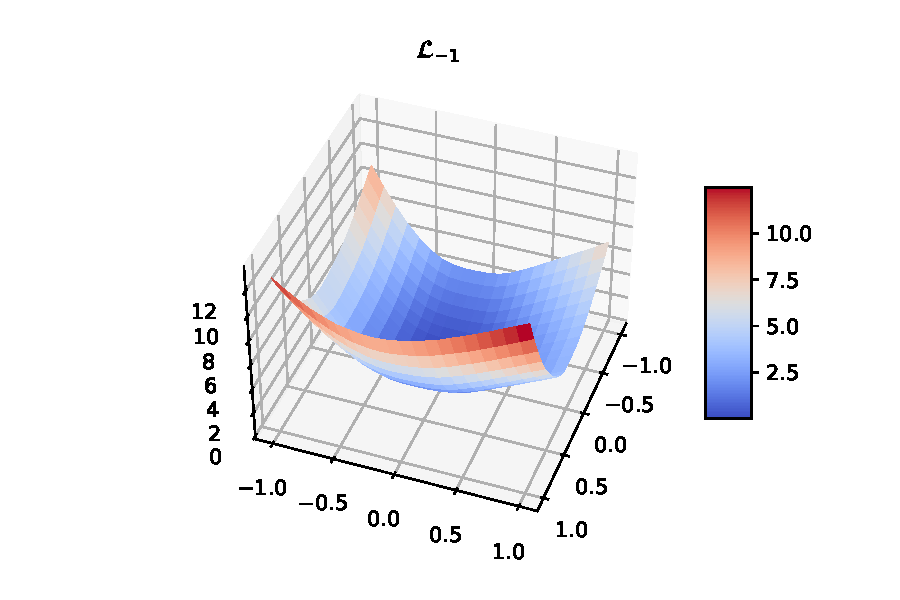
\includegraphics[width=1.2\textwidth]{img/loss_eigen_-1_individ.pdf}
        \column{0.5\textwidth}
        \begin{itemize}
            \item Hessian projection onto top-$d$ eigenvectors
            \item Monte Carlo estimate of $\Delta_k^{emp} = \mathbb{E} \Bigl( \cL_{k+1} - \cL_{k} \Bigr)^2.$
            \item Analytical bound: $\Delta_k^{th} \ge \Delta_k^{emp}$
            \item Detect dataset threshold $k^*$
        \end{itemize}
    \end{columns}
    \bigskip
    \textbf{Main message:} Loss landscape stabilizes after sufficient sample size.
\end{frame}

\begin{frame}{Literature}
    \begin{itemize}
        \item Wu \textit{et al.} (2017): loss landscapes vs dataset size [2]
        \item Sagun \textit{et al.} (2018): Hessian low effective rank [7]
        \item Li \textit{et al.} (2018): visualizing loss surfaces [11]
        \item Ghorbani \textit{et al.} (2019): eigenvalue density analysis [8]
        \item Bousquet \& Elisseeff (2002): stability and generalization bounds [12]
    \end{itemize}
\end{frame}

\begin{frame}{Problem Statement: Hypothesis and Model}
    \begin{block}{Hypothesis}
        Beyond some $k^*$, adding new samples changes the local loss landscape by less than a tolerance $\Delta_{tol}$, i.e.
        $\forall\, k \ge k^* : \; \Delta_k < \Delta_{tol}$.
    \end{block}
    \begin{block}{Model}
        \begin{itemize}
            \item MLP with ReLU activations for $K$-class classification
            \item Empirical loss: $\cL_k(\bw) = \frac1k \sum_{i=1}^k \ell_i(\bw)$
            \item Hessian: $\bH_k(\bw) = \nabla^2_{\bw} \cL_k(\bw)$
        \end{itemize}
    \end{block}
\end{frame}

\begin{frame}{Problem Statement: Quality Criteria}
    \begin{itemize}
        \item Convergence rate: $\Delta_k = O(1/k)$
        \item Theoretical bound via top-$d$ eigenvalues upper-bounds empirical $\Delta_k$
        \item Plateau in eigenvalue differences $\lambda_i^{k+1}-\lambda_i^k$ indicates threshold
    \end{itemize}
\end{frame}

\begin{frame}{Problem Solution: Theoretical Analysis}
    \begin{columns}[c]
        \column{0.4\textwidth}
        \begin{itemize}
            \item Project parameters: $\bw = \bw^* + \bP \btheta$, $\bP = [\be_1, \dots, \be_d]$
            \item Taylor approx: $\cL_k (\bw^* + \bP \btheta) \approx \cL_k (\bw^*) + \tfrac12 \btheta^{\T} \bLambda_k \btheta$
                  \bigskip
                  \bigskip
            \item Bound:
        \end{itemize}
        \column{0.6\textwidth}
        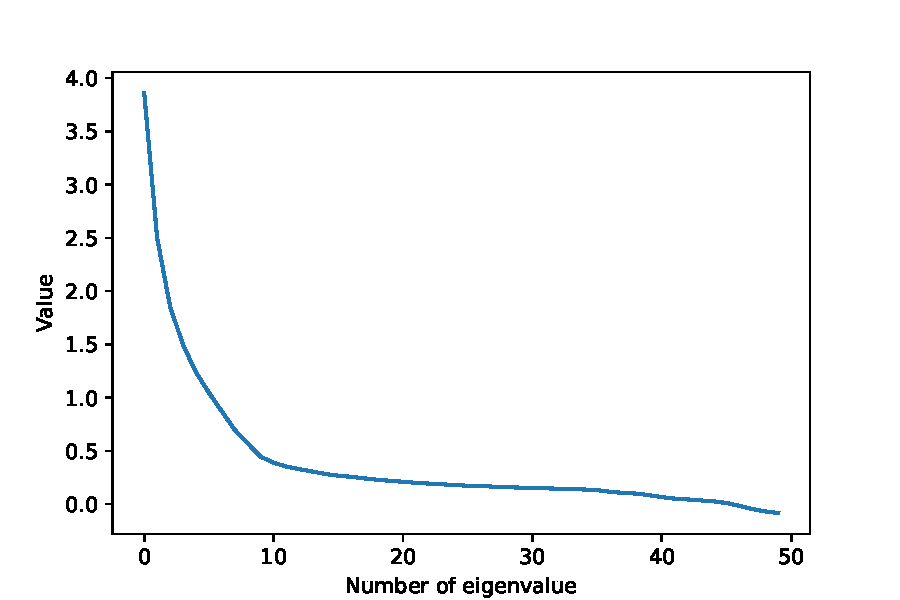
\includegraphics[width=1.0\textwidth]{img/eigenvalues.pdf}
        \vspace{0.5cm}\hspace{1.8cm}\raggedright{\tiny Figure 1: Eigenvalue decay (p.4)}
    \end{columns}
    $$
        \Delta_k \approx
        \frac{\sigma^4}{4}\, \Biggl( 2 \sum_{i=1}^d (\lambda_{k+1}^i - \lambda_k^i)^2
        + \Bigl( \sum_{i=1}^d (\lambda_{k+1}^i - \lambda_k^i) \Bigr)^2 \Biggr).
    $$
\end{frame}

\begin{frame}{Goals of Computational Experiment}
    \begin{itemize}
        \item Datasets: MNIST, Fashion-MNIST (60k train, 10k test)
        \item MLP: 2 hidden layers, $\sim 10^5$ parameters
        \item Subspace dimension $d=10$, Monte Carlo samples $K=64$, $\sigma=1$
        \item Compare empirical $\Delta_k$ vs theoretical bound across $k$
    \end{itemize}

    \begin{figure}
        \centering
        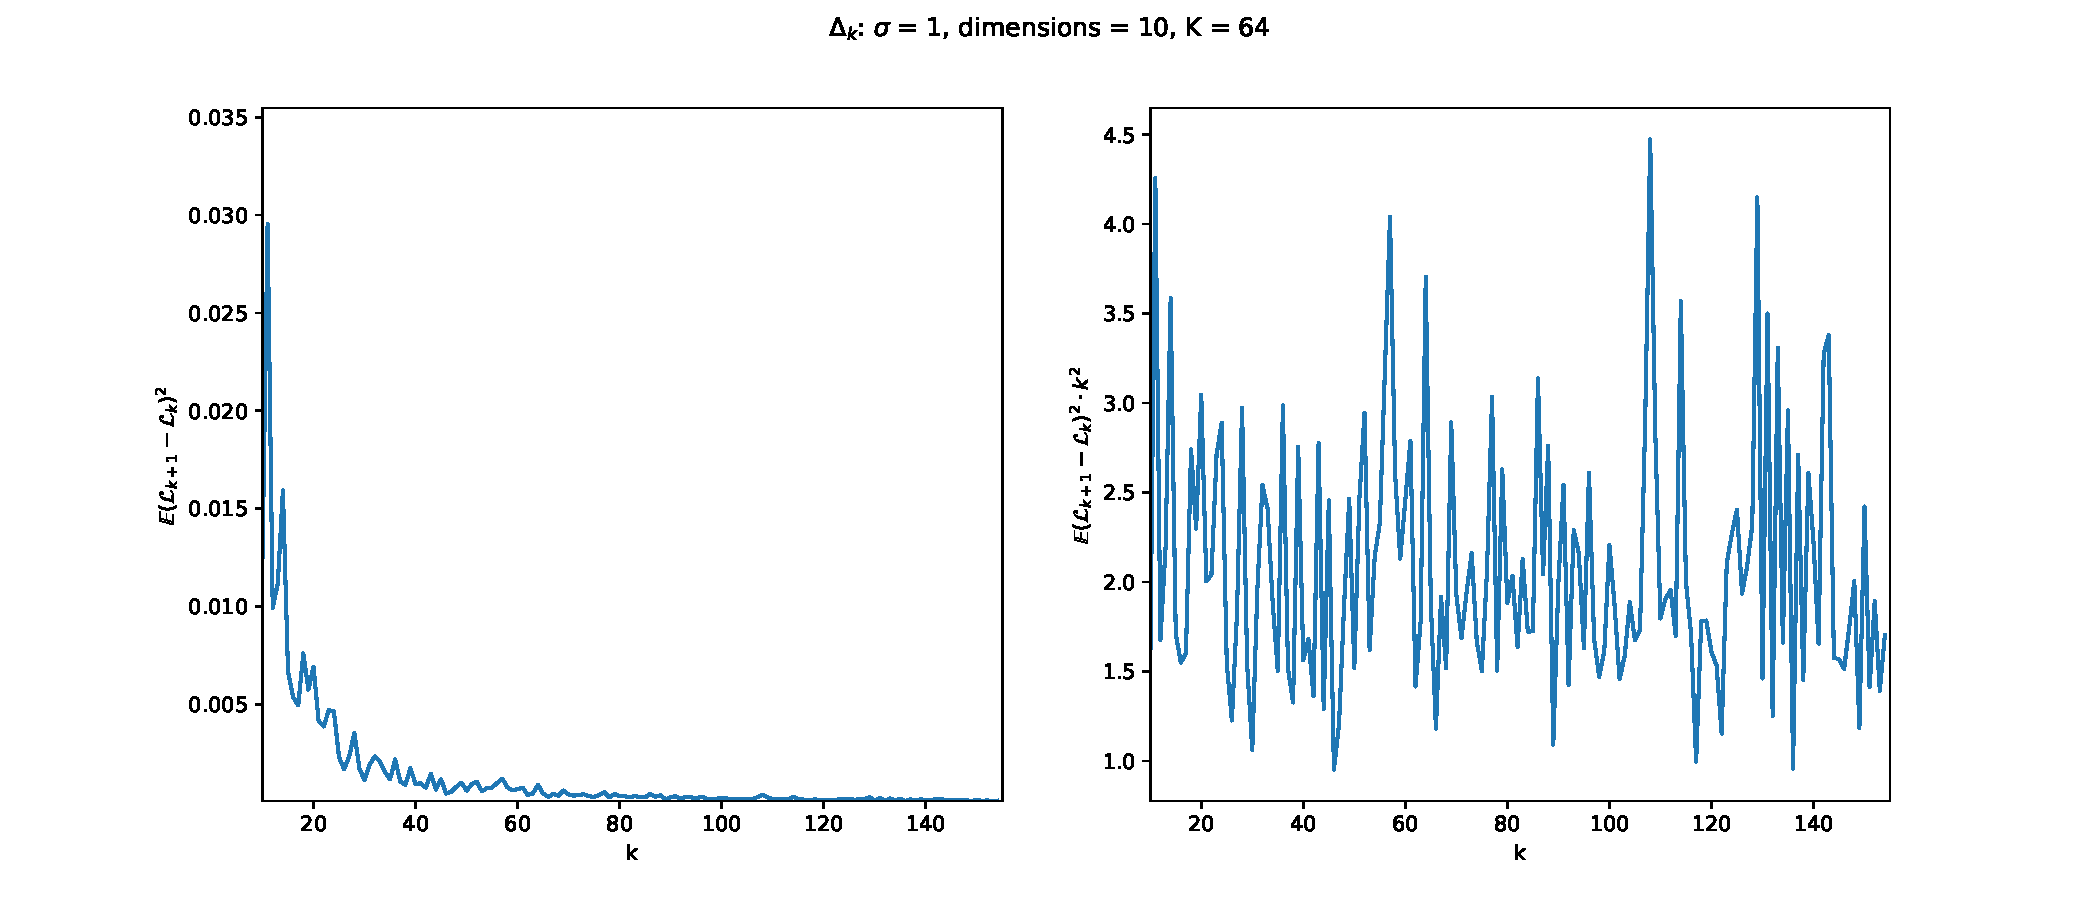
\includegraphics[width=1.05\textwidth,trim=0 17 0 1.5cm,clip]{img/delta_eigen_1_10_64.pdf}
        \caption*{\tiny Figure 8: Monte Carlo $\Delta_k$ vs $k$ and $\Delta_k\cdot k^2$ (p.11)}
    \end{figure}
\end{frame}

\begin{frame}{Error Analysis}
    \begin{itemize}
        \item Empirical $\Delta_k$ consistently below theoretical estimate
        \item Gap due to neglected eigen-modes beyond top-$d$
        \item Monte Carlo variance decreases with sample size $K$
    \end{itemize}

    \begin{figure}
        \centering
        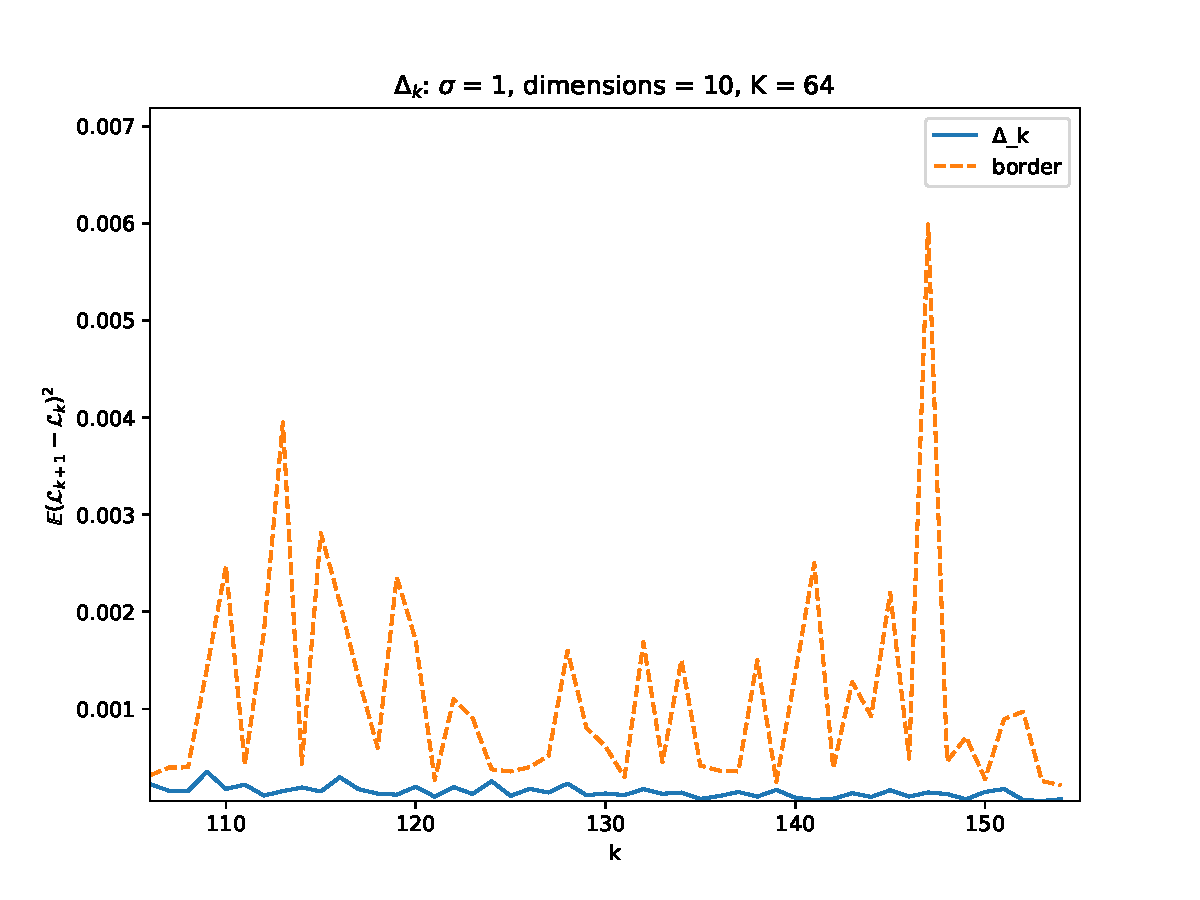
\includegraphics[width=0.7\textwidth]{img/delta_border_1_10_64.pdf}
        \caption*{\tiny Figure 9: Theoretical (dashed) vs empirical (solid) $\Delta_k$ (p.12)}
    \end{figure}
\end{frame}

%\begin{frame}{Models--Datasets--Criteria}
%    \begin{center}
%        \begin{tabular}{|l|l|c|c|}
%            \hline
%            \textbf{Model} & \textbf{Dataset} & \boldmath$d$ & \boldmath$\Delta_{tol}$ \\
%            \hhline{|=|=|=|=|}
%            MLP (2 layers) & MNIST            & 10           & $1\times10^{-4}$        \\
%            \hline
%            MLP (2 layers) & Fashion-MNIST    & 10           & $1\times10^{-4}$        \\
%            \hline
%        \end{tabular}
%    \end{center}
%\end{frame}

\begin{frame}{Results and Conclusions}
    \begin{itemize}
        \item Identified threshold $k$ (MNIST), (Fashion-MNIST)
        \item Loss landscape stabilizes: additional data negligible beyond $k^*$
        \item Hessian-based bound provides reliable upper-bound for $\Delta_k$
        \item Practical guideline for dataset sizing and early stopping
    \end{itemize}
\end{frame}

\end{document}
